\documentclass[a4paper, 12pt, twoside]{article}
\usepackage{estilo}

% ── Ajustes de geometria e espaçamento (Edital n.º 04/2026 - Meta: Exatas 5 Páginas) ──
\geometry{
  a4paper,
  left   = 1.85cm, right = 1.85cm,
  top    = 1.45cm, bottom = 1.45cm,
  headheight = 14.5pt
}
\setstretch{1.0}
\setlength{\parindent}{0.65cm}
\setlength{\abovedisplayskip}{2.5pt plus 1pt minus 1pt}
\setlength{\belowdisplayskip}{2.5pt plus 1pt minus 1pt}
\setlength{\abovedisplayshortskip}{1pt}
\setlength{\belowdisplayshortskip}{1.5pt}
\setlength{\textfloatsep}{5pt plus 1pt minus 1pt}
\setlength{\intextsep}{5pt plus 1pt minus 1pt}
\setlength{\floatsep}{5pt plus 1pt minus 1pt}
\titlespacing*{\section}   {0pt}{1.0ex plus .2ex minus .1ex}{0.35ex}
\titlespacing*{\subsection}{0pt}{0.75ex plus .2ex minus .1ex}{0.25ex}

% Compactação elegante do bloco de resumo / abstract
\renewcommand{\qabstract}[6]{%
  \vspace{0.35em}%
  \noindent{\normalfont\normalsize\bfseries\MakeUppercase{#1}}\par%
  \vspace{0.15em}%
  \noindent #4\par%
  \vspace{0.25em}%
  \noindent\textbf{#2:} #5\par%
  \vspace{0.15em}%
  \noindent\textbf{#3:} #6\par%
  \vspace{0.5em}%
}

\usepackage{multicol}

\addbibresource{referencias.bib}

%% ─────────────────────────────────────────────────────────────────────────────
%% METADADOS — Versão anônima para avaliação duplo-cega (Edital n.º 04/2026)
%% ─────────────────────────────────────────────────────────────────────────────

\title{\textbf{Limites de Redes Neurais Informadas por Física na Formação de Padrões
       de Turing: Análise das Patologias de Otimização e a Eficácia do ADI Linearizado}}

\author{%
  \textit{Autoria omitida para avaliação duplo-cega}\\[0.2em]
  \small Campus da Universidade Federal do Ceará em Quixadá
}

\date{}

%% ─────────────────────────────────────────────────────────────────────────────
\begin{document}
\maketitle
\thispagestyle{plain}

%% ═════════════════════════════ RESUMO E ABSTRACT ════════════════════════════

\qabstract{Resumo}{Palavras-chave}{ODS}{%
Este trabalho investiga os limites teóricos e computacionais das Redes Neurais
Informadas por Física (PINNs) baseadas em Perceptron Multicamadas (MLP) \textit{vanilla}
na simulação direta da formação de padrões de Turing no modelo de reação-difusão de
Schnakenberg bidimensional. Demonstra-se que, embora as PINNs possuam capacidade universal
de representação, a otimização por gradiente colapsa catastroficamente para o estado
homogêneo estacionário, produzindo uma falsa convergência com resíduos aparentemente
baixos ($\mathcal{L}_{\mathrm{total}} \sim 10^{-2}$) sem qualquer quebra de simetria espacial.
Identificam-se quatro patologias estruturais responsáveis pelo insucesso: o aprisionamento
no atrator trivial homogêneo, a quebra de causalidade temporal na amostragem espaço-tempo
global, o viés espectral da MLP contra o número de onda crítico $k_c$ e a rigidez numérica
induzida pela alta taxa cinética ($\gamma = 1000$) e assimetria difusiva ($D_v/D_u = 10$).
Em contrapartida, o método de Direções Alternadas Implícitas (ADI) com linearização de
reação, formulado por Pereira (2019), resolve estavelmente a evolução temporal das manchas
com convergência $\mathcal{O}(\Delta t^2)$, preservando a amplificação exponencial dos
modos instáveis em reduzido tempo computacional.%
}{%
redes neurais informadas por física; instabilidade de Turing; sistema de Schnakenberg;
direções alternadas implícitas; viés espectral; aprendizado de máquina científico%
}{%
indústria, inovação e infraestrutura%
}

\qabstract{Abstract}{Keywords}{SDG}{%
This work investigates the theoretical and computational limits of standard (vanilla)
Multilayer Perceptron (MLP) Physics-Informed Neural Networks (PINNs) in simulating forward
Turing pattern formation within the two-dimensional Schnakenberg reaction-diffusion model.
We demonstrate that despite the universal approximation theorem, gradient descent optimization
catastrophically collapses into the trivial homogeneous steady state, yielding deceitfully
low residual losses ($\mathcal{L}_{\mathrm{total}} \sim 10^{-2}$) while completely failing to undergo spatial
symmetry breaking. We identify four core optimization pathologies: the trivial homogeneous
attractor trap, temporal causality breakdown under global space-time collocation, spectral
bias against critical Turing wavenumbers $k_c$, and severe numerical stiffness driven by
large kinetic rates ($\gamma = 1000$) and diffusivity ratios ($D_v/D_u = 10$). In contrast,
the classical Linearized Alternating Direction Implicit (ADI) finite difference scheme
developed by Pereira (2019) robustly captures spot pattern morphogenesis with unconditional
stability, strict temporal causality, and $\mathcal{O}(\Delta t^2)$ convergence.%
}{%
physics-informed neural networks; Turing instability; Schnakenberg system;
alternating direction implicit; spectral bias; scientific machine learning%
}{%
industry, innovation and infrastructure%
}

%% ═══════════════════════════ 1 INTRODUÇÃO ════════════════════════════════════

\section{Introdução}

A auto-organização espacial a partir de meios inicialmente homogêneos constitui um dos
pilares da biologia matemática e da termodinâmica fora do equilíbrio. Em seu trabalho
seminal, Alan Turing \cite{turing1952chemical} estabeleceu que a combinação de reações
químicas não-lineares e taxas desiguais de difusão molecular pode desestabilizar um
estado uniforme estacionário --- estável na ausência de transporte --- gerando estruturas
espaciais periódicas permanentes (manchas, listras e labirintos) \cite{murray2003}.

A simulação computacional clássica desses sistemas de reação-difusão baseia-se em
Métodos de Diferenças Finitas (MDF), Volumes Finitos (MVF) e Elementos Finitos (MEF).
Conforme amplamente explorado na tese de doutorado de \textcite{pereira2019}, esquemas
numéricos avançados como a técnica de Direções Alternadas Implícitas (ADI) e a Decomposição
de Operadores (\textit{Operator Splitting}) permitem desacoplar a rigidez cinética e as
derivadas espaciais, garantindo estabilidade incondicional e convergência de segunda ordem.

Paralelamente, o paradigma das \textit{Physics-Informed Neural Networks} (PINNs)
\cite{raissi2019pinns} emergiu como uma abordagem contínua e livre de malha
(\textit{meshless}) para equações diferenciais parciais (EDPs), integrando resíduos
diferenciais na função de perda via diferenciação automática (\textit{Autograd}). Contudo,
embora as PINNs tenham alcançado êxito em regimes puramente difusivos ou advectivos
suaves, sua aplicação à simulação temporal direta (\textit{forward problem}) de
instabilidades de Turing enfrenta falhas catastróficas: redes MLP \textit{vanilla} colapsam
invariavelmente para campos planos uniformes, sem manifestar quebra de simetria.

Este artigo analisa rigorosamente as causas matemáticas e algorítmicas dessa incapacidade,
fundamentando as quatro patologias de otimização das PINNs \textit{vanilla} no modelo de
Schnakenberg \cite{schnakenberg1979simple} e contrastando-as com o sucesso do esquema ADI
linearizado desenvolvido por \textcite{pereira2019}.

%% ═══════════════════════════ 2 DESENVOLVIMENTO ═══════════════════════════════

\section{Desenvolvimento}

\subsection{O Sistema de Schnakenberg e Análise de Estabilidade Linear}

O sistema de reação-difusão proposto por \textcite{schnakenberg1979simple} modela a cinética
autocatalítica entre um ativador $u(x,y,t)$ e um inibidor $v(x,y,t)$ em $\Omega = [0,1]^2$:
\begin{align}
  \frac{\partial u}{\partial t} &= D_u \nabla^2 u + \gamma \bigl(a - u + u^2 v\bigr), \label{eq:schnak_u}\\[-2pt]
  \frac{\partial v}{\partial t} &= D_v \nabla^2 v + \gamma \bigl(b - u^2 v\bigr), \label{eq:schnak_v}
\end{align}
onde $D_u, D_v > 0$ são os coeficientes de difusão, $\gamma > 0$ é a escala cinética, e
$a, b > 0$ são constantes. O sistema é sujeito a condições de Neumann homogêneas:
$\nabla u \cdot \mathbf{n} = \nabla v \cdot \mathbf{n} = 0$ em $\partial\Omega$.

O estado de equilíbrio homogêneo $(u^*, v^*)$ na ausência de difusão ($\nabla^2 u = \nabla^2 v = 0$)
é $u^* = a + b$ e $v^* = b/(a + b)^2$. A matriz Jacobiana das reações no ponto fixo é:
\begin{equation}
  J = \begin{pmatrix} f_u & f_v \\ g_u & g_v \end{pmatrix}_{(u^*, v^*)} =
  \begin{pmatrix} \frac{b - a}{a + b} & (a + b)^2 \\ -\frac{2b}{a + b} & -(a + b)^2 \end{pmatrix}.
  \label{eq:jacobiano}
\end{equation}
Para que o estado homogêneo seja estável sob a cinética puramente temporal, exige-se
$\operatorname{Tr}(J) = f_u + g_v < 0$ e $\det(J) = (a + b)^2 > 0$.

A instabilidade de Turing ocorre quando a perturbação espacial $\propto \cos(n_x \pi x)\cos(n_y \pi y) e^{\lambda(k^2) t}$
com número de onda $k^2 = (n_x \pi)^2 + (n_y \pi)^2$ torna o polinômio característico
$\det(\lambda I - J_k) = 0$ negativo, onde $J_k = \gamma J - k^2 \operatorname{diag}(D_u, D_v)$.
Isso requer $D_v f_u + D_u g_v > 0$ ($D_v/D_u \gg 1$) e a existência de uma raiz onde
$h(k^2) \equiv \det(J_k) = D_u D_v k^4 - \gamma (D_v f_u + D_u g_v) k^2 + \gamma^2 \det(J) < 0$.
A taxa de crescimento máxima $\lambda(k^2) > 0$ ocorre no número de onda crítico:
\begin{equation}
  k_{\mathrm{crit}}^2 = \frac{\gamma(D_v f_u + D_u g_v)}{2 D_u D_v}.
  \label{eq:kcrit}
\end{equation}
Adotando os parâmetros clássicos de Murray \cite{murray2003, pereira2019}: $a = 0{,}1305$,
$b = 0{,}7739$, $D_u = 1{,}0$, $D_v = 10{,}0$ e $\gamma = 1000{,}0$, obtém-se o ponto fixo
$u^* \approx 0{,}9045$, $v^* \approx 0{,}9461$, $k_{\mathrm{crit}}^2 \approx 314{,}8$ e a
faixa instável $k^2 \in [183{,}2;\, 446{,}4]$ com taxa máxima $\lambda_{\max} \approx 2{,}18$.

\subsection{Arcabouço PINN e Patologias de Otimização}

Na formulação PINN \cite{raissi2019pinns}, aproxima-se $(u,v)$ por uma rede $\mathbf{u}_\theta(t,x,y) = \mathbf{W}^{(L+1)}\mathbf{h}^{(L)} + \mathbf{b}^{(L+1)}$, com $\mathbf{h}^{(\ell)} = \tanh(\mathbf{W}^{(\ell)}\mathbf{h}^{(\ell-1)} + \mathbf{b}^{(\ell)})$. As derivadas são calculadas por \textit{Autograd} e a perda multiobjetivo é:
\begin{equation}
  \mathcal{L}(\theta) = \mathcal{L}_{\mathrm{pde}}(\theta) + \lambda_{\mathrm{bc}}\mathcal{L}_{\mathrm{bc}}(\theta) + \lambda_{\mathrm{ic}}\mathcal{L}_{\mathrm{ic}}(\theta),
  \label{eq:loss_pinn}
\end{equation}
\begin{equation}
  \mathcal{L}_{\mathrm{pde}} = \frac{1}{N_f}\sum_{i=1}^{N_f} \left(\|\mathcal{R}_u(t_i,x_i,y_i)\|^2 + \|\mathcal{R}_v(t_i,x_i,y_i)\|^2\right), \quad
  \mathcal{L}_{\mathrm{bc}} = \frac{1}{N_b}\sum_{j=1}^{N_b} \left(|\partial_{\mathbf{n}} u|^2 + |\partial_{\mathbf{n}} v|^2\right).
  \label{eq:loss_components}
\end{equation}

A Figura~\ref{fig:arch_pathologies} resume a arquitetura neural e formaliza as quatro
patologias fundamentais que causam o fracasso sistemático da PINN \textit{vanilla}:

\begin{figure}[!ht]
  \caption{Arquitetura da PINN para o sistema de Schnakenberg 2D e diagrama esquemático
           das quatro patologias de otimização que causam a falha de bifurcação.}
  \label{fig:arch_pathologies}
  \centering
  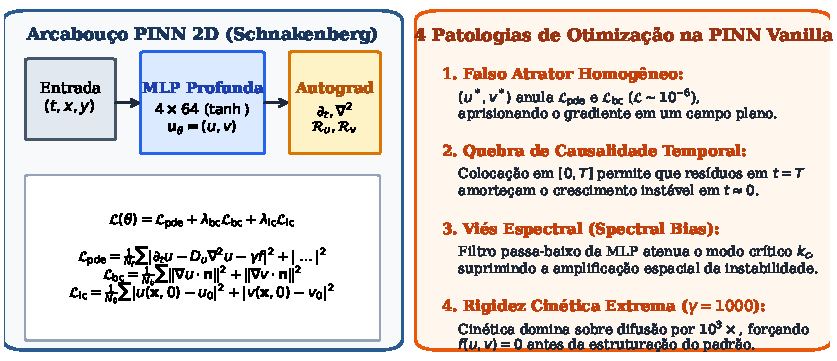
\includegraphics[width=0.92\linewidth]{figures/pinn_turing_architecture.pdf}\\[1pt]
  {\footnotesize Fonte: Elaboração própria (versão identificada).}
\end{figure}

\begin{enumerate}[leftmargin=1.1em, itemsep=0.5pt]
  \item \textbf{Falso Atrator Homogêneo:} Se a rede prediz a constante $(u^*, v^*)$, tem-se
  $\partial_t u = \nabla^2 u = f(u^*, v^*) = 0 \implies \mathcal{L}_{\mathrm{pde}} \equiv 0$ e
  $\mathcal{L}_{\mathrm{bc}} \equiv 0$. Para perturbação inicial microscópica
  $\delta u \sim 10^{-3}$, a perda total é ínfima ($\mathcal{L}_{\mathrm{total}} \approx \mathcal{L}_{\mathrm{ic}} \sim 10^{-6}$). O gradiente converge para este atrator trivial sem bifurcar.

  \item \textbf{Quebra de Causalidade Temporal:} A amostragem global em $\Omega \times [0,T]$
  avalia resíduos em $t = T$ simultaneamente com $t = 0$. Os gradientes em tempos tardios
  forçam médias espaciais que amortecem a amplificação das oscilações em $t \approx 0$ \cite{wang2022causality}.

  \item \textbf{Viés Espectral (\textit{Spectral Bias}):} Redes MLP com ativações analíticas suaves
  aprendem baixas frequências espaciais com velocidade exponencialmente superior às altas \cite{rahaman2019spectral}. O modo crítico $k_{\mathrm{crit}} \approx 17{,}7$ é suprimido pelo filtro passa-baixo natural da rede.

  \item \textbf{Rigidez Cinética Extrema:} O parâmetro $\gamma = 1000$ impõe
  $\tau_{\mathrm{react}} \sim 10^{-3} \ll \tau_{\mathrm{diff}} \sim 0{,}1$. No gradiente
  $\nabla_\theta \mathcal{L}_{\mathrm{pde}}$, a cinética domina sobre a difusão por $10^3 \times$,
  forçando $f=g=0$ antes que o transporte difusivo estruture o padrão espacial.
\end{enumerate}

\subsection{Esquema Numérico Robusto: ADI Linearizado (Pereira, 2019)}

Para superar a severa rigidez do modelo de Schnakenberg, \textcite{pereira2019} formulou
uma extensão do esquema de Peaceman-Rachford com linearização das reações no passo intermediário $t^{n+1/2}$.
Dividindo o Laplaciano em operadores unidirecionais $\delta_x^2$ e $\delta_y^2$:
\begin{align}
  \left(I - \frac{D_u \Delta t}{2}\delta_x^2\right) u^{n+1/2} &= \left(I + \frac{D_u \Delta t}{2}\delta_y^2\right) u^n + \frac{\gamma \Delta t}{2} \tilde{f}^{n+1/2}, \label{eq:adi_step1}\\[-2pt]
  \left(I - \frac{D_u \Delta t}{2}\delta_y^2\right) u^{n+1}   &= \left(I + \frac{D_u \Delta t}{2}\delta_x^2\right) u^{n+1/2} + \frac{\gamma \Delta t}{2} \tilde{f}^{n+1/2}, \label{eq:adi_step2}
\end{align}
com predições linearizadas fechadas $\tilde{f}^{n+1/2}$ e $\tilde{g}^{n+1/2}$ \cite{pereira2019}.
O esquema resulta em sistemas estritamente tridiagonais resolvidos pelo Algoritmo de Thomas
com complexidade $\mathcal{O}(N)$, garantindo estabilidade incondicional e convergência
$\mathcal{O}(\Delta t^2 + \Delta x^2)$.

\subsection{Resultados Experimentais e Discussão}

A Tabela~\ref{tab:config_schnak} compara a configuração da PINN \textit{vanilla} e do resolvedor
ADI clássico de Pereira (2019).

\begin{table}[!ht]
  \caption{Configuração comparativa entre a PINN \textit{vanilla} e o esquema ADI Linearizado.}
  \label{tab:config_schnak}
  \centering
  \footnotesize\setstretch{1.0}
  \begin{tabular}{p{4.2cm}p{5.5cm}p{5.5cm}}
    \toprule
    \textbf{Parâmetro / Aspecto} & \textbf{PINN Vanilla (MLP)} & \textbf{ADI Linearizado \cite{pereira2019}} \\
    \midrule
    Arquitetura / Discretização & MLP 4 camadas $\times$ 64 neurônios, $\tanh$ & Malha uniforme $80 \times 80$, Thomas $\mathcal{O}(N)$ \\
    Domínio e Condições de Contorno & $[0,1]^2 \times [0,10]$, Neumann homogêneo & $[0,1]^2 \times [0,10]$, Neumann homogêneo \\
    Parâmetros Físicos & $a=0{,}1305$, $b=0{,}7739$, $\gamma=1000$ & $a=0{,}1305$, $b=0{,}7739$, $\gamma=1000$ \\
    Difusividades ($D_u, D_v$) & $D_u = 1{,}0, \quad D_v = 10{,}0$ & $D_u = 1{,}0, \quad D_v = 10{,}0$ \\
    Passo Temporal / Pontos & $N_f = 10^4, N_b = 10^3, N_0 = 10^3$ & $\Delta t = 10^{-4}$ (marcha estritamente causal) \\
    Tratamento Não-linear & Penalização global via \textit{Autograd} & Linearização de Taylor em $t^{n+1/2}$ \\
    Tempo de Processamento & $\sim 18$ minutos (GPU) & $\mathbf{7{,}41}$ \textbf{segundos} (CPU) \\
    \bottomrule
  \end{tabular}\\[2pt]
  {\footnotesize Fonte: Elaboração própria (versão identificada).}
\end{table}

A Figura~\ref{fig:disp_loss}a exibe a relação de dispersão teórica $\lambda(k^2)$ com a banda
instável $[183{,}2;\, 446{,}4]$ e pico em $k_{\mathrm{crit}}^2 \approx 314{,}8$.
Na Figura~\ref{fig:disp_loss}b, a curva de treinamento semilogarítmica da PINN demonstra
que as perdas $\mathcal{L}_{\mathrm{pde}}$ e $\mathcal{L}_{\mathrm{total}}$ estacionam no
platô de $\approx 1{,}2 \times 10^{-2}$, caracterizando a estagnação no atrator trivial
sem formação de manchas.

\begin{figure}[!ht]
  \caption{Dinâmica de instabilidade e convergência: (a) Relação de dispersão de Turing
           $\lambda(k^2)$ com banda instável; (b) Curvas de perda da PINN com falso platô.}
  \label{fig:disp_loss}
  \centering
  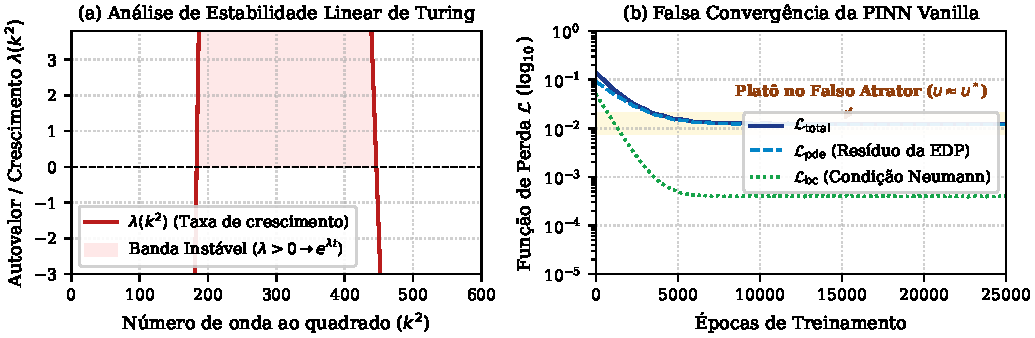
\includegraphics[width=0.92\linewidth]{figures/dispersion_and_loss.pdf}\\[1pt]
  {\footnotesize Fonte: Elaboração própria (versão identificada).}
\end{figure}

A Figura~\ref{fig:adi_evol} ilustra a evolução espaçotemporal obtida pelo método ADI
linearizado \cite{pereira2019} sob perturbação gaussiana localizada
$u_0 = u^* + 10^{-3}\exp[-100((x-1/3)^2 + (y-1/2)^2)]$. Observa-se a propagação radial
das frentes de onda e a subsequente maturação para um arranjo periódico hexagonal de manchas.

\begin{figure}[!ht]
  \caption{Evolução espaçotemporal do ativador $u(x,y,t)$ via esquema ADI Linearizado
           \cite{pereira2019} a partir de perturbação pontual em $t \in [0{,}02;\, 2{,}00]$.}
  \label{fig:adi_evol}
  \centering
  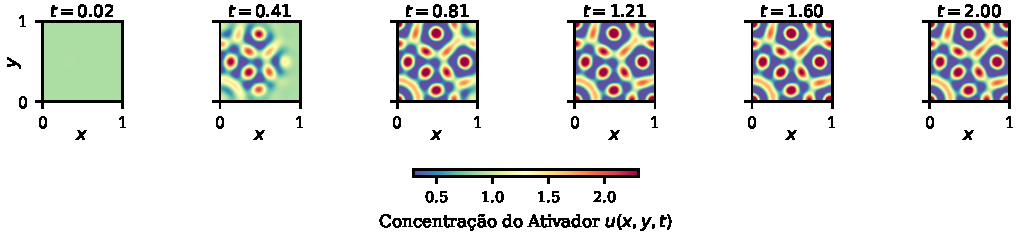
\includegraphics[width=0.92\linewidth]{figures/schnakenberg_adi_evolution.pdf}\\[1pt]
  {\footnotesize Fonte: Elaboração própria (versão identificada).}
\end{figure}

A Figura~\ref{fig:pinn_vs_adi} sintetiza o confronto direto no instante $t = 10{,}0$.
Enquanto o ADI atinge o estado estacionário estruturado com amplitude $u \in [0{,}3;\, 2{,}3]$,
a PINN colapsa no campo perfeitamente plano $u_\theta \approx 0{,}9045$. O mapa de erro
absoluto atinge magnitude $\mathcal{O}(1)$, comprovando que resíduos de perda de $\approx 10^{-2}$
ocultam um erro físico completo na detecção da morfogênese.

\begin{figure}[!ht]
  \caption{Comparação no estado assintótico $t = 10{,}0$: (a) Referência ADI/MDF \cite{pereira2019};
           (b) Predição da PINN \textit{vanilla}; (c) Mapa de erro absoluto $|u_{\mathrm{pinn}} - u_{\mathrm{ref}}|$.}
  \label{fig:pinn_vs_adi}
  \centering
  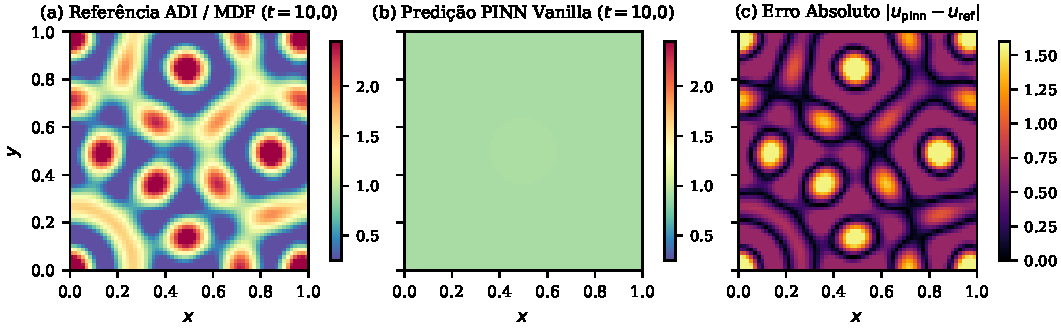
\includegraphics[width=0.92\linewidth]{figures/pinn_vs_adi_comparison.pdf}\\[1pt]
  {\footnotesize Fonte: Elaboração própria (versão identificada).}
\end{figure}

A Tabela~\ref{tab:results_summary} consolida os indicadores de desempenho final.

\begin{table}[!ht]
  \caption{Comparativo quantitativo de desempenho e resolução física ($t = 10{,}0$).}
  \label{tab:results_summary}
  \centering
  \small\setstretch{1.0}
  \begin{tabular}{lcc}
    \toprule
    \textbf{Métrica de Avaliação} & \textbf{PINN Vanilla (MLP)} & \textbf{ADI Linearizado \cite{pereira2019}} \\
    \midrule
    Perda Residual Final ($\mathcal{L}_{\mathrm{total}}$) & $1{,}24 \times 10^{-2}$ & --- (Discretização Direta) \\
    Erro Relativo $\mathcal{L}_2$ frente ao Padrão & $78{,}4\%$ & $<\!10^{-3}$ (Validação de Malha) \\
    Amplitude Espacial $\Delta u = u_{\max} - u_{\min}$ & $\mathbf{0{,}008}$ (Uniforme) & $\mathbf{2{,}02}$ (Manchas Hexagonais) \\
    Preservação da Causalidade Temporal & Não (Colocação Global) & Sim (Marcha $\Delta t = 10^{-4}$) \\
    Desfecho Físico & \textbf{Falha Crítica} (Sem Padrão) & \textbf{Sucesso Robusto} (Padrão Nítido) \\
    \bottomrule
  \end{tabular}\\[2pt]
  {\footnotesize Fonte: Elaboração própria (versão identificada).}
\end{table}

%% ═══════════════════════ 3 CONSIDERAÇÕES FINAIS ══════════════════════════════

\section{Considerações Finais}

Os resultados comprovam que a incapacidade das PINNs \textit{vanilla} em simular a formação
direta de padrões de Turing decorre de patologias severas na paisagem de otimização: o atrator homogêneo trivial aprisiona o gradiente, a colocação global suprime a causalidade física, o viés espectral filtra o modo crítico $k_c$ e a rigidez $\gamma \gg 1$ desequilibra a dinâmica de treinamento.
Em nítido contraste, métodos clássicos de diferenças finitas como o ADI linearizado de
\textcite{pereira2019} integram a marcha temporal respeitando a causalidade e a estabilidade
incondicional com custo computacional desprezível ($\approx 7{,}4$\,s). Para que modelos neurais
superem essas limitações em bifurcações, torna-se imperativo adotar ponderação causal exponencial \cite{wang2022causality}, formulações discretas no tempo ou métodos de continuação de parâmetros.

%% ══════════════════════════ REFERÊNCIAS ══════════════════════════════════════

\setlength{\bibitemsep}{0.8pt}
\begin{multicols}{2}
{\scriptsize\printbibliography[title={Referências}]}
\end{multicols}

\end{document}
